\documentclass[12pt]{article}
\usepackage[margin = 0.9in, top=0.8in]{geometry}
\usepackage{graphicx}
\usepackage{textgreek}
\usepackage{amsmath}
\usepackage{amsfonts}
\usepackage{mathtools}
\usepackage{amssymb}
\usepackage{float}
\usepackage{subcaption}
\usepackage{hyperref}
\usepackage{grffile}
\graphicspath{{./2/images},{./2/data}, {./}}

\title{CS 754 - Advanced Image Processing\\Assignment 3 - Report}
\author{Shaan ul Haque - 180070053\\Mantri Krishna Sri Ipsit - 180070032}
\newcommand{\norm}[1]{\left\lVert #1 \right\rVert}
\begin{document}

\maketitle

\section*{Question 1}
\subsection*{1.a}
We would like the loss function defined by:
\begin{equation*}
    f_N(\beta) = \frac{|| \boldsymbol{y-X}\beta||^2_2}{2N}
\end{equation*}
to be strictly convex. For this we would like that the double derivative matrix, $\nabla^2 f(\beta) = \boldsymbol{X^TX}/N$, wrt to $\beta$ have all its eigenvalues be positive or be away from zero. Since $\boldsymbol{X} \in \boldsymbol{R^{p \times N}}$, the rank of $\boldsymbol{X^TX}$ is equal to min\{N,p\} which makes the matrix rank deficit.\\
To relax the notion of convexity, we allow the function to be strictly convex in only some subset $\boldsymbol{C} \subset \boldsymbol{R^p}$. Thus, a function in strictly convex at $\beta^*$ wrt to a set $\boldsymbol{C}$ if:
\begin{equation*}
    \frac{v^T\nabla^2 f(\beta)v}{||v||^2_2} \geq \gamma \ \forall \ \textrm{non-zero} \ v \ \in \ \boldsymbol{C}
\end{equation*}
which, for our case gives (also called as \textit{restricted eigenvalues}):
\begin{equation*}
    \frac{v^T\boldsymbol{X^TX}v}{N||v||^2_2} \geq \gamma \ \forall \ \textrm{non-zero} \ v \ \in \ \boldsymbol{C}
\end{equation*}
Thus, we would like the minimum value of the LHS in the above equation to be greater than or equal to $\gamma$. Since the minimum value of the LHS is the minimum eigenvalue ($\lambda_{min}$) with the corresponding eigenvector constrained in the subset $\boldsymbol{C}$, we can also write the above equation as:
\begin{equation*}
    \lambda_{min} \geq \gamma \ \forall \ \textrm{non-zero} \ v \ \in \ \boldsymbol{C}
\end{equation*}
This is called as restricted eigenvalue condition.
\subsection*{1.b}
It is given that $\hat{\nu}$ is the minimizer of the equation:
\begin{equation*}
    G(\hat{\nu}) = \frac{||\boldsymbol{y-X}(\beta^*+\hat{\nu})||^2_2}{2N}+\lambda_N||(\beta^*+\hat{\nu})||_1
\end{equation*}
Thus, from the above assumption we can write $G(\hat{\nu}) \leq G(0)$
\subsection*{1.c}
Using the inequality obtained in previous part:
\begin{equation*}
    \frac{||\boldsymbol{y-X}(\beta^*+\hat{\nu})||^2_2}{2N}+\lambda_N||(\beta^*+\hat{\nu})||_1 \leq \frac{||\boldsymbol{y-X}\beta^*||^2_2}{2N}+\lambda_N||\beta^*||_1
\end{equation*}
Now since $\boldsymbol{y} = \boldsymbol{X}\beta^*+\boldsymbol{w}$, we substitute $\boldsymbol{w}$ in the above inequality to get:
\begin{equation*}
    \frac{||\boldsymbol{w}-\boldsymbol{X}\hat{\nu}||^2_2}{2N} - \frac{||\boldsymbol{w}||^2_2}{2N} \leq \lambda_N(||\beta^*||_1 - ||(\beta^*+\hat{\nu})||_1)
\end{equation*}
opening the brackets, we get:
\begin{equation*}
    \frac{(\boldsymbol{w}-\boldsymbol{X}\hat{\nu})^T(\boldsymbol{w}-\boldsymbol{X}\hat{\nu})}{2N} - \frac{\boldsymbol{w}^T\boldsymbol{w}}{2N} \leq \lambda_N(||\beta^*||_1 - ||(\beta^*+\hat{\nu})||_1)
\end{equation*}
which after simplification gives:
\begin{equation*}
    -\frac{\boldsymbol{w}^T\hat{\nu}\boldsymbol{X}}{N} + \frac{\hat{\nu}^T\boldsymbol{X}^T\boldsymbol{X}\hat{\nu}}{2N}\leq \lambda_N(||\beta^*||_1 - ||(\beta^*+\hat{\nu})||_1)
\end{equation*}
The above inequality after shifting terms right and left becomes our required expression:
\begin{equation*}
    \frac{||\boldsymbol{X}\hat{\nu}||^2_2}{2N}\leq \frac{\boldsymbol{w}^T\boldsymbol{X}\hat{\nu}}{N} + \lambda_N(||\beta^*||_1 - ||(\beta^*+\hat{\nu})||_1)
\end{equation*}
\subsection*{1.d}
Since the expression $\frac{\boldsymbol{w}^T\boldsymbol{X}\hat{\nu}}{N}$ can also be written as $\frac{\hat{\nu}^T\boldsymbol{X}^T\boldsymbol{w}}{N}$ because this quantity is a scalar and transpose of scalar is same as the scalar, we get:
\begin{equation*}
    \hat{\nu}^T\boldsymbol{X}^T\boldsymbol{w} = <\hat{\nu}, \boldsymbol{X}^T\boldsymbol{w}>
\end{equation*}
Let for the sake of clarity assume $\boldsymbol{X}^T\boldsymbol{w} = \boldsymbol{y}$. Thus, the dot product becomes:
\begin{equation*}
    <\hat{\nu}, \boldsymbol{y}> = \sum_{i=1}^{p}\hat{\nu}_iy_i \leq \sum_{i=1}^{p}|\hat{\nu}_iy_i| \leq max_i\{|y_i|\}\sum_{i=1}^{p}|\hat{\nu}_i|
\end{equation*}
Writing the above equation in norm form we get ($||a||_\infty = max_n{|a_n|}$):
\begin{equation*}
    <\hat{\nu}, \boldsymbol{y}> = \sum_{i=1}^{p}\hat{\nu}_iy_i  \leq ||\boldsymbol{y}||_\infty||\hat{\nu}||_1
\end{equation*}
Hence, after dividing by N both sides we get:
\begin{equation*}
    \frac{\hat{\nu}^T\boldsymbol{X}^T\boldsymbol{w}}{N} \leq \frac{||\boldsymbol{X}^T\boldsymbol{w}||_\infty}{N}||\hat{\nu}||_1
\end{equation*}
Let $x_S \in  R^{|S|}$ denote the subvector indexed by elements of set S, with $x_{S^c}$ defined in an analogous manner.\\
For the other term we have $\beta^*_{S_c} = 0$, as $\beta^*$ is assumed to be |S|-sparse vector and:
\begin{equation*}
    ||\beta^*+\hat{\nu}||_1 = ||\beta^*_{S}+\hat{\nu}_{S}||_1+||\hat{\nu}_{S^c}||_1 \geq ||\beta^*_{S}||_1-||\hat{\nu}_{S}||_1+||\hat{\nu}_{S^c}||_1
\end{equation*}
Using above two inequalities, we can obtain eq. 11.22 as:
\begin{equation*}
    \frac{||\boldsymbol{X}\hat{\nu}||^2_2}{2N}\leq \frac{||\boldsymbol{X}^T\boldsymbol{w}||_\infty}{N}||\hat{\nu}||_1 + \lambda_N(||\hat{\nu}_{S}||_1-||\hat{\nu}_{S^c}||_1)
\end{equation*}
\subsection*{1.e}
Firstly, it is assumed that $\frac{||\boldsymbol{X}^T\boldsymbol{w}||_\infty}{N} \leq \frac{\lambda_N}{2}$. Using this:
\begin{equation*}
    \frac{||\boldsymbol{X}\hat{\nu}||^2_2}{2N} \leq \frac{\lambda_N}{2}(||\hat{\nu}_{S}||_1-||\hat{\nu}_{S^c}||_1) + \lambda_N(||\hat{\nu}_{S}||_1+||\hat{\nu}_{S^c}||_1)  
\end{equation*}
\begin{equation*}
    = \frac{3}{2}\lambda_N||\hat{\nu}_{S}||_1-\frac{1}{2}\lambda_N||\hat{\nu}_{S^c}||_1 \leq \frac{3}{2}\lambda_N||\hat{\nu}_{S}||_1 \leq \frac{3}{2}\sqrt{k}\lambda_N||\hat{\nu}||_2 \ \textrm{(using Cauchy-Schwartz inequality)}
\end{equation*}
\subsection*{1.f}
Using the restricted Eigenvalue condition and assuming the lasso error $\hat{\beta} - \beta^*$ is in the set $\boldsymbol{C}$ (defined in part a), we have:
\begin{equation*}
    \frac{v^T\boldsymbol{X^TX}v}{||v||^2_2} \geq \gamma \ \forall \ \textrm{non-zero} \ v \ \in \ \boldsymbol{C}
\end{equation*}
which gives:
\begin{equation*}
    \frac{||\boldsymbol{X}\hat{v}||_2^2}{2N} = \frac{\hat{v}^T\boldsymbol{X^TX}\hat{v}}{2N} \geq \frac{\gamma ||\hat{v}||^2_2}{2}
\end{equation*}
From the bound derived in previous part we have:
\begin{equation*}
    \frac{\gamma ||\hat{v}||^2_2}{2} \leq \frac{||\boldsymbol{X}\hat{\nu}||^2_2}{2N} \leq  \frac{3}{2}\sqrt{k}\lambda_N||\hat{\nu}||_2 
\end{equation*}
Thus, we have:
\begin{equation*}
    ||\hat{\beta} - \beta^*||_2 = ||\hat{v}||_2 \leq \frac{3}{\gamma}\sqrt{\frac{k}{N}}\sqrt{N}\lambda_N 
\end{equation*}
\subsection*{1.g}
It is an assumption that we make in order to prove the cone constraint that $||\hat{\nu}_{S^c}||_1 \leq \alpha||\hat{\nu_S}||_1$. Specifically, we used the inequality to prove the bound in part e. Using the inequality in part e, we have:
\begin{equation*}
    \frac{||\boldsymbol{X}\hat{\nu}||^2_2}{2N} \leq \frac{3}{2}\lambda_N||\hat{\nu}_{S}||_1-\frac{1}{2}\lambda_N||\hat{\nu}_{S^c}||_1
\end{equation*}
Since the LHS is always greater than or equal to 0, we get:
\begin{equation*}
    0 \leq \frac{3}{2}\lambda_N||\hat{\nu}_{S}||_1-\frac{1}{2}\lambda_N||\hat{\nu}_{S^c}||_1 \Longrightarrow  ||\hat{\nu}_{S^c}||_1 \leq 3||\hat{\nu}_{S}||_1 \ \textrm{(Cone constraint)}
\end{equation*}
\subsection*{1.h}
In the first part we saw that in order to minimize the loss function it must be strictly convex whereas in practice it is convex in some direction while non-concave in others. Thus, we relaxed the condition and allowed strict convexity only in a subset $\boldsymbol{C} \subset \boldsymbol{R}^p$. The lasso regression constraint that $||\beta||_1 \leq R$ with or without regularization leads the subset to be cone, i.e, $||\hat{\nu_S}||_1 \leq \alpha||\hat{\nu}_{S^c}||_1$.
\subsection*{1.i}
In both the theorems we are required to calculate the minimum eigenvalue of our dictionary matrix but in this theorem our search for the minimum eigenvalue is deterministic, i.e.,   in a set with cone constraint and moreover here we do not need the explicit calculation of the RIC. One fascinating thing to observe here is that this theorem also emphasizes on the interaction of the dictionary with noise vector, greater the correlation greater is the error whereas theorem 3 doesn't take any such thing into account.  Apart from this, the rate this theorem achieves, including the logarithmic factor, is known to be minimax optimal, meaning that it cannot be substantially improved upon by any estimator.\\
The biggest drawback of this theorem is that it doesn't consider compressible signals. The sparsity constraint for the sensed signal is very tight and does not allow room for signals which are less sparse but some elements are very small. Theorem 3 handles such situation well. 
\subsection*{1.j}
The common thread between `Dantzig selector' and the LASSO is accounting for the interaction of dictionary with the noise vector in the error bound. For `Dantzig selector' the maximum correlation $||A^Te||_{\infty}$ is assumed to be less than some constant $\lambda$. A similar kind of constraint was assumed for LASSO also, as assumed for proving the sub part 1.e. 
\subsection*{1.k}
Square-root lasso's biggest advantage is that without knowing or pre-estimating the noise variance $\sigma^2$, we can get near-oracle performance. The regression parameter in the lasso regression depends on the noise variance whose estimation in certain cases might be non-trivial. Moreover, in all $l_2$ error constraints, noise is assumed to be Gaussian in nature. But the theorem in paper doesn't require the knowledge of the noise variance, on top of that it doesn't even assume noise to be Gaussian in nature.

\section*{Question 2}
The original images of the slices used are as follows:
\begin{figure}[ht]
	\centering
	\begin{minipage}[bt]{0.3\linewidth}
		\centering
		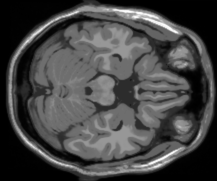
\includegraphics[scale=0.5]{slice_50.png}
		\caption{Slice 50}
	\end{minipage}
	\begin{minipage}[bt]{0.3\linewidth}
		\centering
		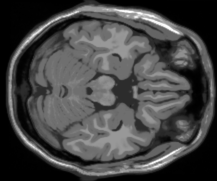
\includegraphics[scale=0.5]{slice_51.png}
		\caption{Slice 51}
	\end{minipage}
	\begin{minipage}[bt]{0.3\linewidth}
		\centering
		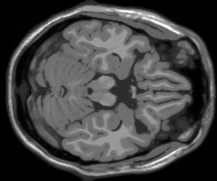
\includegraphics[scale=0.5]{slice_52.png}
		\caption{Slice 52}
	\end{minipage}
\end{figure}
\subsection*{Part a}
Here the tomographic reconstruction is performed using the \textbf{Filtered Backprojection} using the \textbf{Ram-Lak} filter. The reconstruction results for slices 50 and 51 are as follows:
\begin{figure}[ht]
	\centering
	\begin{minipage}[bt]{0.5\linewidth}
		\centering
		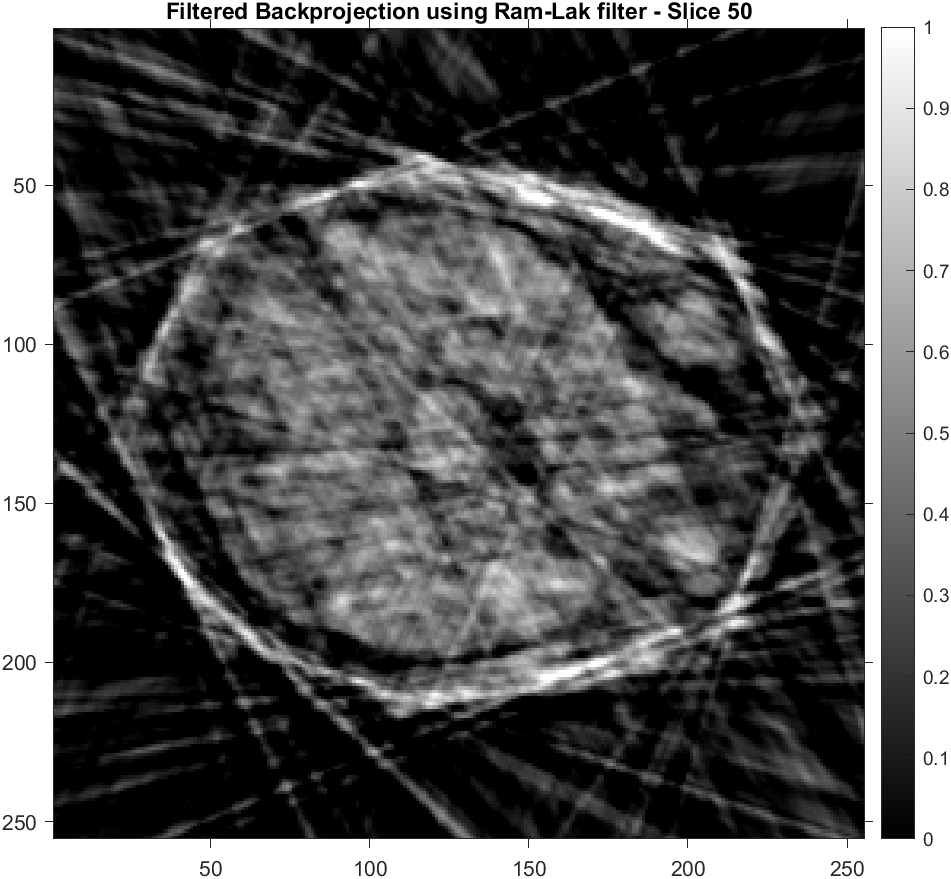
\includegraphics[scale=0.25]{a_50.png}
		\caption{Ram-Lak FBP - Slice 50}
	\end{minipage}
	\begin{minipage}[bt]{0.4\linewidth}
		\centering
		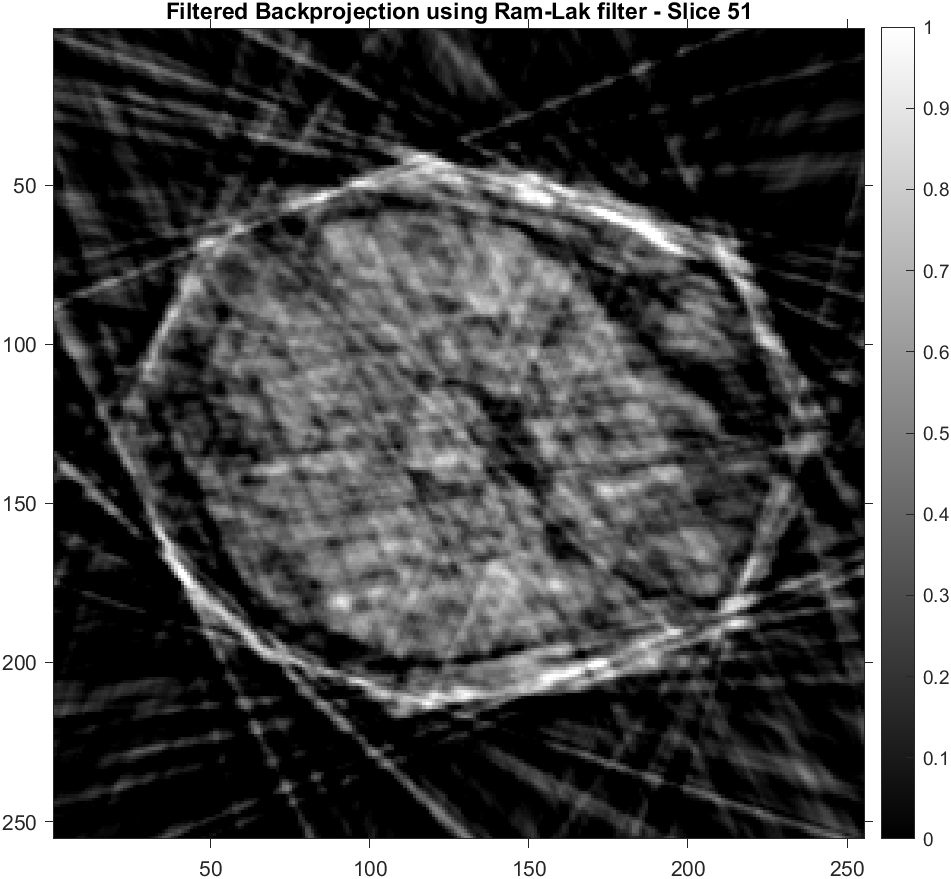
\includegraphics[scale=0.25]{a_51.png}
		\caption{Ram-Lak FBP - Slice 51}
	\end{minipage}
\end{figure}
\subsection*{Part b}
Here the tomographic reconstruction is performed by using the \textbf{Independent Compressive Sensing} based reconstruction for each slice by solving an optimization problem of the form
$$J(x) = \norm{y - Ax}_2^2 + \lambda \norm{x}_1$$
The reconstruction results for slices 50 and 51 are as follows:
\begin{figure}[ht]
	\centering
	\begin{minipage}[bt]{0.5\linewidth}
		\centering
		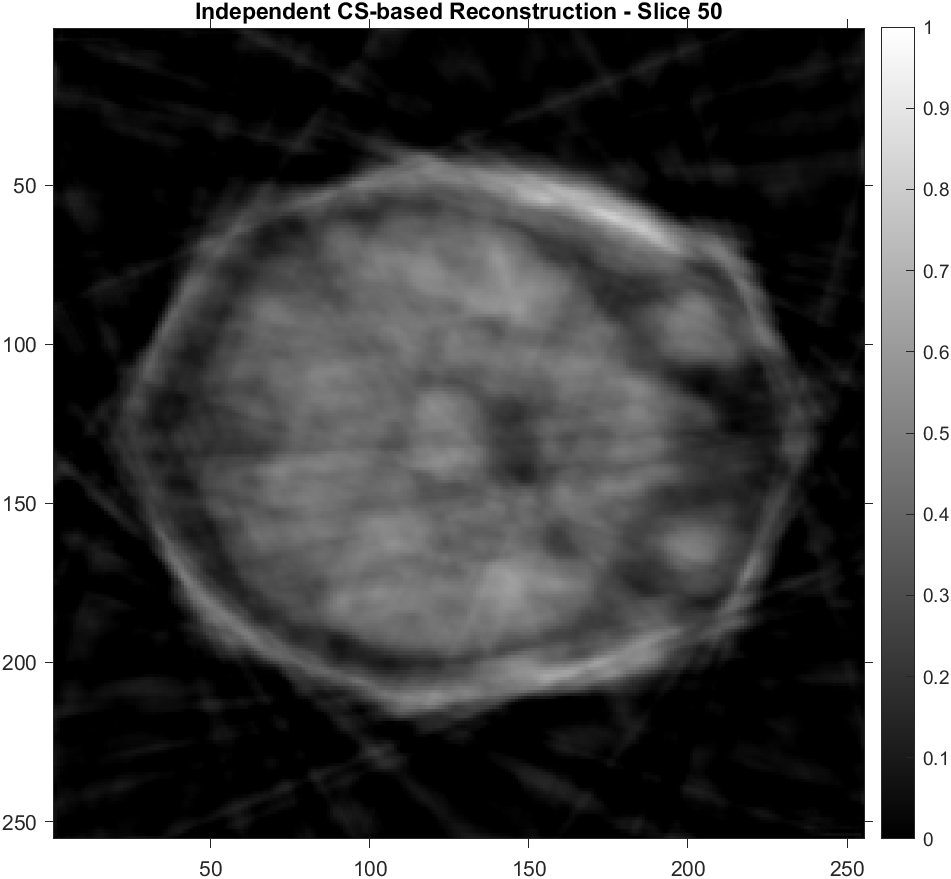
\includegraphics[scale=0.25]{b_50.png}
		\caption{Independent CS - Slice 50}
	\end{minipage}
	\begin{minipage}[bt]{0.4\linewidth}
		\centering
		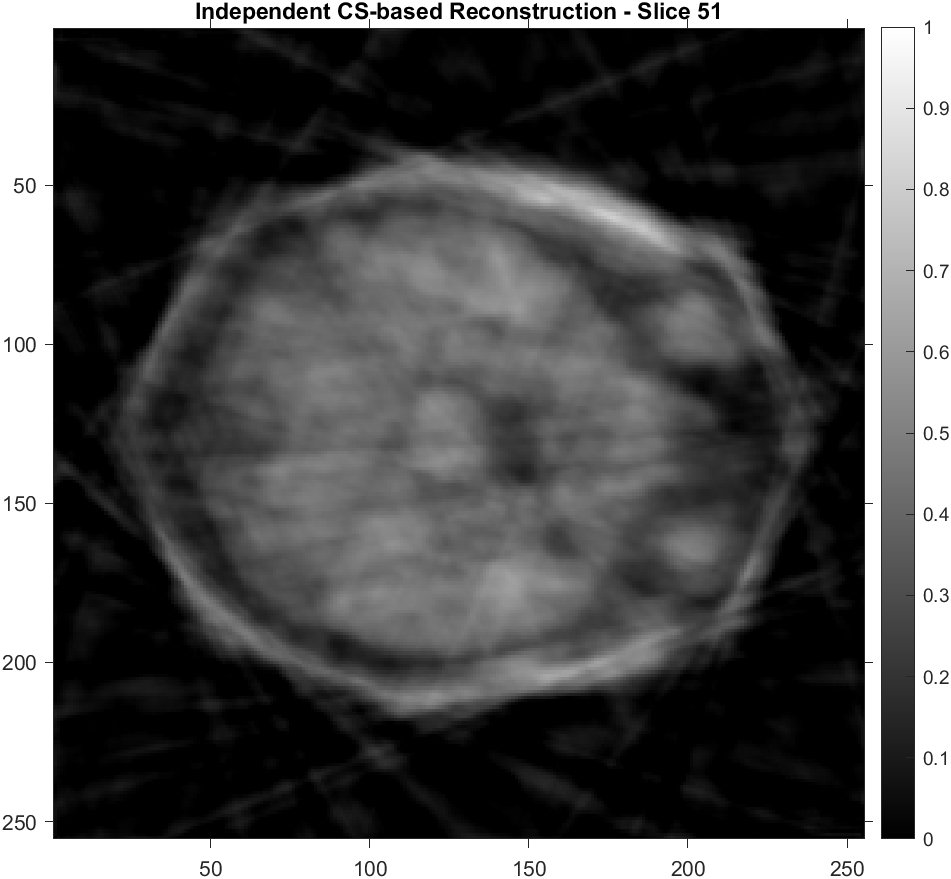
\includegraphics[scale=0.25]{b_51.png}
		\caption{Independent CS - Slice 51}
	\end{minipage}
\end{figure}
\subsection*{Part c}
Here the tomographic reconstruction is performed by using the \textbf{Coupled Compressive Sensing} based reconstruction by solving an optimization problem of the form:
$$J\bigg(\begin{bmatrix}
\beta_1 \\ \Delta \beta_1
\end{bmatrix}\bigg) = \norm{\begin{bmatrix}
	y_1\\y_2
	\end{bmatrix} - \begin{bmatrix}
	R_1U & 0\\
	R_2U & R_2U
	\end{bmatrix} \begin{bmatrix}
	\beta_1 \\ \Delta \beta_1
	\end{bmatrix}}_2^2 + \lambda \norm{\begin{bmatrix}
	\beta_1 \\ \Delta \beta_1
	\end{bmatrix}}_1$$
The reconstruction results for slices 50 and 51 are as follows:
\begin{figure}[ht]
	\centering
	\begin{minipage}[bt]{0.5\linewidth}
		\centering
		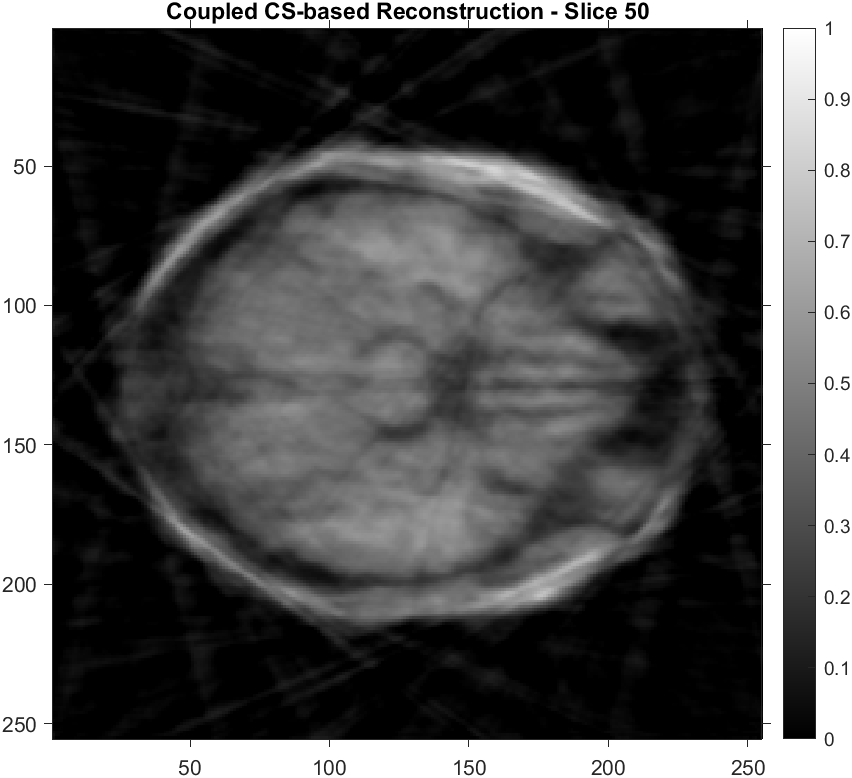
\includegraphics[scale=0.25]{c_50.png}
		\caption{Coupled CS - Slice 50}
	\end{minipage}
	\begin{minipage}[bt]{0.4\linewidth}
		\centering
		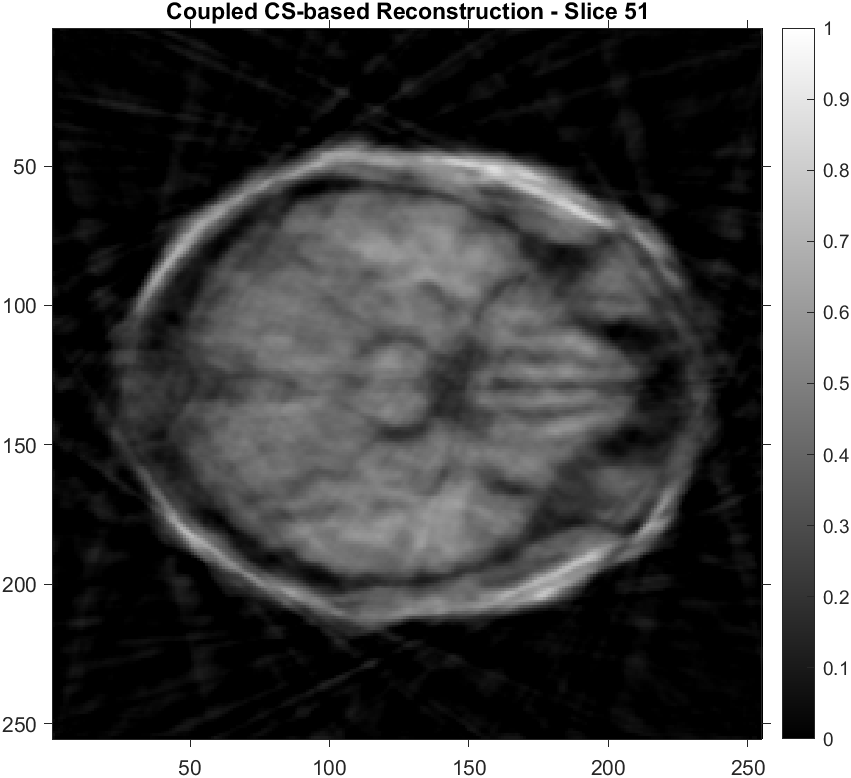
\includegraphics[scale=0.25]{c_51.png}
		\caption{Coupled CS - Slice 51}
	\end{minipage}
\end{figure}
\subsection*{Part d}
Here the tomographic reconstruction is performed by using the \textbf{Coupled Compressive Sensing} based reconstruction \textbf{using 3 slices} by solving an optimization problem of the form:
$$J\bigg(\begin{bmatrix}
\beta_1 \\ \Delta \beta_1 \\ \Delta \beta_2
\end{bmatrix}\bigg) = \norm{\begin{bmatrix}
	y_1\\y_2\\y_3
	\end{bmatrix} - \begin{bmatrix}
	R_1U & 0 & 0\\
	R_2U & R_2U & 0\\
	R_3U & 0 & R_3U
	\end{bmatrix} \begin{bmatrix}
	\beta_1 \\ \Delta \beta_1\\ \Delta \beta_2
	\end{bmatrix}}_2^2 + \lambda \norm{\begin{bmatrix}
	\beta_1 \\ \Delta \beta_1\\ \Delta \beta_2
	\end{bmatrix}}_1$$
Here 
\begin{itemize}
	\item  $y_1, y_2, y_3$ are the radon transforms of 3 slices $x_1, x_2, x_3$ under consideration.
	\item $\beta_1$ is the 2D-DCT of first slice $x_1$, vectorized.
	\item $\beta_1 + \Delta \beta_1$ is the 2D-DCT of second slice $x_2$, vectorized.
	\item $\beta_1 + \Delta \beta_2$ is the 2D-DCT of second slice $x_3$, vectorized.
	\item $R_1$ is the radon transform matrix for the random angles used to compute tomographic projections of $x_1$.
	\item $R_2$ is the radon transform matrix for the random angles used to compute tomographic projections of $x_2$.
	\item $R_3$ is the radon transform matrix for the random angles used to compute tomographic projections of $x_3$.
\end{itemize}
The reconstruction results for slices 50, 51 and 52 are as follows:
\begin{figure}[ht]
	\centering
	\begin{minipage}[bt]{0.3\linewidth}
		\centering
		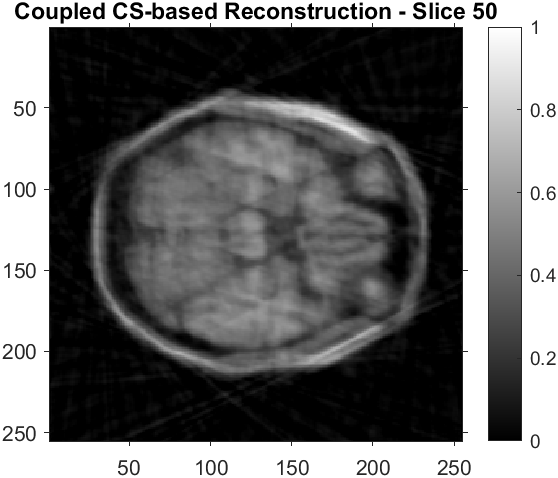
\includegraphics[scale=0.5]{d_50.png}
		\caption{3 CS - Slice 50}
	\end{minipage}
	\begin{minipage}[bt]{0.3\linewidth}
		\centering
		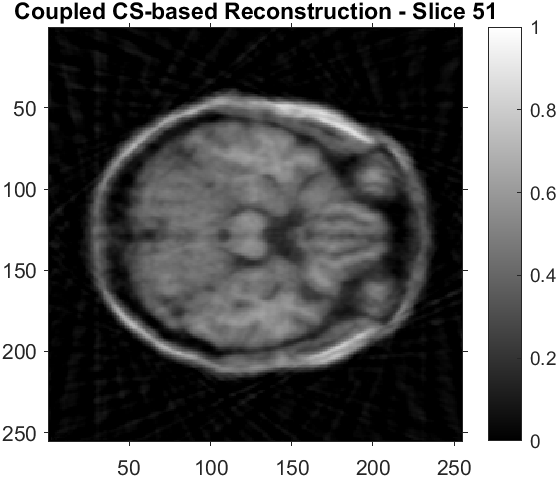
\includegraphics[scale=0.5]{d_51.png}
		\caption{3 CS - Slice 51}
	\end{minipage}
	\begin{minipage}[bt]{0.3\linewidth}
		\centering
		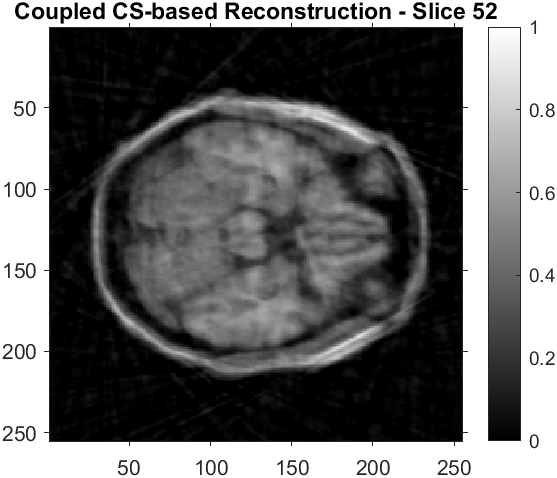
\includegraphics[scale=0.5]{d_52.png}
		\caption{3 CS - Slice 52}
	\end{minipage}
\end{figure}


\section*{Question 3}
For the sake of notational simplicity, denote $R(\rho, \theta)$ as the radon transform of $g(x, y)$ at a translation $\rho$ and at an angle $\theta$.
$$R(\rho, \theta) = \int\limits_{-\infty}^\infty \int \limits_{-\infty}^\infty g(x, y) \, \delta(x \cos\theta  + y \sin \theta - \rho)\: dx\,dy$$
\subsection*{Part a}
\begin{eqnarray*}
	R\big(g(x-x_0, y-y_0)\big)(\rho, \theta) &=& \int\limits_{-\infty}^\infty \int \limits_{-\infty}^\infty g(x-x_0, y-y_0)\,\delta(x \cos\theta  + y \sin \theta - \rho)\: dx\,dy\\\\
	\text{Replace } x \rightarrow u+x_0, y \rightarrow v+y_0&&\\
	&=& \int\limits_{-\infty}^\infty \int \limits_{-\infty}^\infty g(u, v)\, \delta\bigg(u\cos \theta + v \sin\theta - \big(\rho - x_0\cos\theta - y_0\sin\theta\big)\bigg)\: dx\,dy\\
	&=& R\big(g(u, v)\big)(\rho - x_0\cos\theta - y_0\sin\theta, \theta)\\
	&=& R\big(g(x, y)\big)(\rho - x_0\cos\theta - y_0\sin\theta, \theta)
\end{eqnarray*}

\subsection*{Part b}
$$g'(r, \psi) = g(r, \psi - \psi_0)$$
Consider the radon transform in polar coordinates:
$$R(g)(\rho, \theta) = \int \limits_{0}^{2\pi} \int \limits_{0}^\infty g(r, \psi)\, \delta\bigg(r\cos(\psi-\theta) - \rho\bigg)\: r\,dr\,d\psi$$
\vspace{2cm}
\begin{center}
	\textit{Please turn over}
\end{center}

Now, 
\begin{eqnarray*}
	R(g')(\rho, \theta) &=& \int \limits_{0}^\infty \int \limits_{0}^{2\pi} g'(r, \psi) \: \delta\bigg(r \cos(\psi - \theta) - \rho\bigg) \: r\, dr\, d\psi\\
	&=& \int \limits_{0}^\infty \int \limits_{0}^{2\pi} g(r, \psi - \psi_0) \: \delta\bigg(r \cos(\psi  - \theta) - \rho\bigg) \: r\, dr\, d\psi\\
	\text{Replace }\psi \rightarrow \psi_0 + \alpha &&\\
	&=& \int \limits_0^\infty \int \limits_{-\psi_0}^{2\pi-\psi_0}g(r, \alpha)\, \delta\bigg(r \cos(\alpha + \psi_0 - \theta) - \rho\bigg) \: r\,dr\,d\alpha\\
	&=& \int \limits_0^\infty \int \limits_{0}^{2\pi} g(r, \alpha)\, \delta\bigg(r \cos \big(\alpha - (\theta - \psi_0)\big) - \rho\bigg)\: r \,dr\,d\alpha\\
	\text{Replace } \alpha \rightarrow \psi&&\\
	&=&	\int \limits_0^\infty \int \limits_{0}^{2\pi} g(r, \psi)\, \delta\bigg(r \cos \big(\psi - (\theta - \psi_0)\big) - \rho\bigg)\: r \,dr\,d\psi\\
	&=& R(g)(\rho, \theta - \psi_0)
\end{eqnarray*}
\vspace{3cm}
\begin{center}
\textit{Please turn over}
\end{center}
\newpage
\subsection*{Part c}
The convolution of two signals $f(x, y)$ and $k(x, y)$ is given by:
$$(f * k)(x, y) = \int \limits_{-\infty}^\infty \int \limits_{-\infty}^\infty f(u, v) k(x-u, y-v)\: dudv$$

The radon transform of the convolution will be
\begin{eqnarray*}
	R_\theta(f*k) &=& \int \limits_{-\infty}^\infty \int \limits_{-\infty}^ \infty (f*k)(x, y)\, \delta(x \cos \theta + y \sin \theta - \rho)\: dxdy\\
	&=& \int \limits_{-\infty}^\infty \int \limits_{-\infty}^ \infty \int \limits_{-\infty}^\infty \int \limits_{-\infty}^ \infty f(u, v) k(x-u, y-v)\, \delta(x \cos \theta + y \sin \theta - \rho)\: dudv\: dxdy\\
	\text{Replace } x-u \rightarrow a, y-v \rightarrow b&&\\
	&=& \int \limits_{-\infty}^\infty \int \limits_{-\infty}^ \infty \int \limits_{-\infty}^\infty \int \limits_{-\infty}^ \infty  f(u, v) k(a, b) \, \delta((u+a)\cos\theta + (v+b)\sin \theta - \rho)\: dudv\: dadb\\
	&=& \int \limits_{-\infty}^\infty \int \limits_{-\infty}^ \infty \int \limits_{-\infty}^\infty \int \limits_{-\infty}^ \infty f(u, v) k(a, b) \, dudvdadb \int \limits_{-\infty}^\infty \delta(u\cos\theta + v\sin\theta - \sigma)\\
	&&\hskip 12em\delta(a\cos\theta + b\sin\theta - (\rho-\sigma))\: d\sigma\\
	&=& \int \limits_{-\infty}^\infty \bigg(\int \limits_{-\infty}^\infty\int \limits_{-\infty}^\infty f(u,v) \delta(u\cos\theta + v\sin\theta - \sigma)\, dudv\bigg)\\
	&&\bigg(\int \limits_{-\infty}^\infty\int \limits_{-\infty}^\infty k(a, b)\,\delta(a\cos\theta + b\sin\theta - (\rho-\sigma))\,dadb \bigg)\, d\sigma\\
	&=&  \int \limits_{-\infty}^\infty R(f)(\sigma, \theta) \, R(k)(\rho - \sigma, \theta)\: d\sigma\\
	&=& R_\theta(f) * R_\theta(k)
\end{eqnarray*}


\section*{Question 4}
Mutual coherence is defined as:
\begin{equation*}
    \mu(\boldsymbol{A)} = max_{i, j, i \neq j}\frac{|\boldsymbol{A}_i^T\boldsymbol{A}_j|}{||\boldsymbol{A}_i||_2||\boldsymbol{A}_j||_2} = max_{i, j, i \neq j}|\boldsymbol{A}_i^T\boldsymbol{A}_j| 
\end{equation*}
where, the second equality assumes unit normalized columns.
Now coming at RIC:
\begin{equation*}
    \delta_S = max\{\lambda_{max}-1, 1-\lambda_{min}\}
\end{equation*}
where, $\lambda_{max}$ and $\lambda_{min}$ are the maximum and minimum Eigenvalue of $\boldsymbol{X} = \boldsymbol{A_{\Gamma}^TA_{\Gamma}}$. Here subscript $\Gamma$ denotes only those indices retained in column of the matrix where the sparse vector $\boldsymbol{\theta}$ has non-zero elements. 
Gershgorin theorem states that every Eigenvalue of a matrix B lies between:
\begin{equation*}
    B_{ii}-r_i \leq \lambda \leq B_{ii}+r_i
\end{equation*}
where $B_{ii}$ is the diagonal element at ith row while $r_i$ is the sum of off-diagonal elements. Using this we have:
\begin{equation*}
    \boldsymbol{X}_{ii}-r_i \leq \lambda_{max} \leq \boldsymbol{X}_{ii}+r_i
\end{equation*}
Now, since every (i,j) element of $\boldsymbol{X}$ is the dot product between the ith and jth column of $\boldsymbol{A_{\Gamma}}$ and $\mu(\boldsymbol{A)}$ is maximum among them barring the special case when i=j where the value of $\boldsymbol{X}_{ii} = 1$, we get:
\begin{equation*}
     \lambda_{max} \leq 1+\mu(\boldsymbol{A)}(S-1) \Longrightarrow \lambda_{max}-1 \leq 1+\mu(\boldsymbol{A)}(S-1)
\end{equation*}
where, the RHS is the consequence of only $|\Gamma| \leq S$ columns in $\boldsymbol{A_{\Gamma}}$. Now using the other side of inequality for $\lambda_{min}$, we get:
\begin{equation*}
  1-\mu(\boldsymbol{A)}(S-1) \leq \lambda_{min} \Longrightarrow 1-\lambda_{min} \leq \mu(\boldsymbol{A)}(S-1)
\end{equation*}
Using the above two inequalities, we get:
\begin{equation*}
  max\{\lambda_{max}-1, 1-\lambda_{min}\} \leq \mu(\boldsymbol{A)}(S-1) \Longrightarrow \delta_S \leq \mu(\boldsymbol{A)}(S-1)
\end{equation*}

\section*{Question 5}
\begin{itemize}
    \item \textbf{Title:} Tomographic reconstruction of the ionosphere using ground-based GPS data in the Australian region.
    \item \textbf{Venue:}  Physics Department, La Trobe University, Bundoora, Vic 3086, Australia
    \item \textbf{Year of publication of the paper:} 2015
\end{itemize}
\subsection*{Mathematical Problem}
The reconstruction plane is discretized into two-dimensional pixels as shown in Fig. Usually, the grid of these two dimensional boxes is subdivided equidistantly with height and angular spacing. For the present study the grid boxes are 10 km in height and $1^\circ$ (~100 km) in width as shown in Fig. By assuming that the electron density is constant in each pixel, the TEC(Total Electron Content) along the ray path can be represented as a finite sum of shorter integrals along segments of the ray path length. Mathematically this can be expressed as:
\begin{equation*}
    \boldsymbol{STEC_i} = \sum_{j=1}^{M}n_jd_{ij}+e_j
\end{equation*}
where, $\boldsymbol{STEC_i}$ is the measurement for the ith projection, $n_j$ is the electron density in the jth pixel, $d_{ij}$ is the measurement constant, $e_j$ is the noise while M is the total number of pixels along each projection. In matrix form, it can be written as:
\begin{equation*}
    \boldsymbol{Y}_{T\times1} = \boldsymbol{D}_{T\times N}\boldsymbol{N}_{N\times1} + \boldsymbol{E_{T\times1}}
\end{equation*}
where $\boldsymbol{Y}$ is a column of T measurements, $\boldsymbol{N}$ is a column of the M unknown $n_j$s, $\boldsymbol{E}$ is a column of T values representing the error due to data noise and discretization, $\boldsymbol{D}$ is a T × M matrix with $d_{ij}$ being the length of link i that lies in pixel j, and thus $d_{ij}$ is 1 if the ith ray traverses through the jth pixel and 0 otherwise. Due to high precision in measurements, the model is simplified into:
\begin{equation*}
    \boldsymbol{Y}_{T\times1} = \boldsymbol{D}_{T\times N}\boldsymbol{N}_{N\times1}
\end{equation*}
\begin{figure}[H]
  % will center the figure.
  \centering
  % include graphics (can include eps, jpg, pdf ...)
  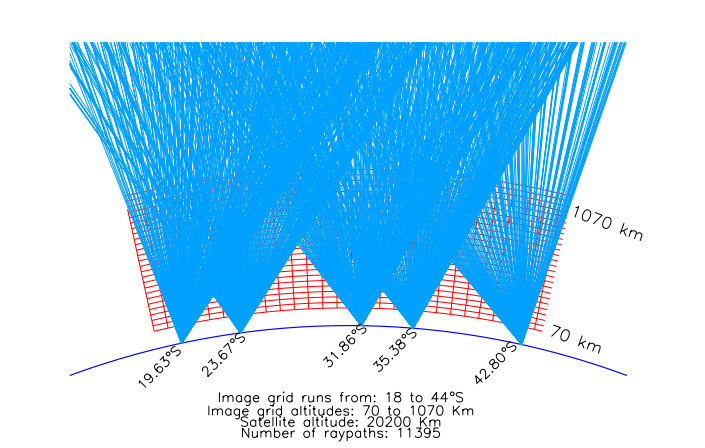
\includegraphics[scale=0.75]{tomo.png}  % change scale factor to re-size the image.
  % give a caption.
  \caption{Experimental setup}
  % a label to refer to the figure
  \label{fig:1}
\end{figure}
\subsection*{Method of optimization}
One of the most commonly used inversion techniques is called algebraic reconstruction technique (ART). The ART algorithm, which can converge quickly in an iterative fashion compared to other reconstruction algorithms, is the preferable algorithm to use for ionospheric reconstruction in a region of interest with a limited widely spaced number of receivers, like the GPS receiver network in the Australian region. Due to these
preferences, the ART algorithm has been used in this paper.
\begin{equation*}
    \boldsymbol{N}^{k+1} = \boldsymbol{N}^{k} + \lambda_k\frac{STEC_i - \sum_{j=1}^Md_{ij}n_j^k}{\sum_{j=1}^Md_{ij}d_{ij}}\boldsymbol{D}_i
\end{equation*}
where $\boldsymbol{D}_i$ is the ith row of $\boldsymbol{D}$, k is iteration number, and $\lambda_k$ is the relaxation parameter. The relaxation parameter ensures that the correction remains stable, and it is a real number usually confined to the interval $0 < \lambda_k < 2$ . The value of $\lambda_k$ is chosen to be the same for all iterations. In this case $\lambda_k$ = 0.005 had been used for all iterations.

\end{document}
